Den Beginn dieser Arbeit bildet die Erläuterung einiger Grundbegriffe und Technologien, die im weiteren Verlauf genutzt werden.

\subsection{Künstliche Intelligenz (KI)}
\label{section:ki}


\subsection{Job Shop Scheduling?}
% ??? oder Scheduling allgemein?

\subsection{Traveling Salesman Problem (TSP)}
\label{sec:grundlagen_tsp}
\todo{NP-schwer erwähnen?!}

Das Traveling Salesman Problem, im deutschen auch bekannt als das Problem des Handlungsreisenden, ist ein schon sehr altes Problem der theoretischen Informatik. Es handelt sich dabei um ein kombinatorisches Optimierungsproblem. Die Problemstellung selbst ist dabei sehr einfach erklärt: Ein Handlungsreisender möchte eine Menge von Stationen mit einer möglichst kurzen Reisestrecke besuchen. Jede Station soll dabei genau einmal besucht werden und die erste Station ist gleich der letzten, sodass ein Kreis entsteht. Ziel der Optimierung ist es also, die best mögliche Reihenfolge der zu besuchenden Orte zu finden (ein beispielhaftes Problem ist in Abb. \ref{fig:tsp_deutschland} dargestellt). \cite{travelingSalesman}

\begin{figure}[H]
    \centering
    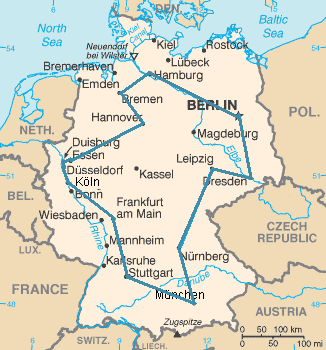
\includegraphics[width=0.5\textwidth]{images/TSP_Deutschland_3.png}
    \caption{TSP Beispiel - Beste Reiseroute durch die 15 größten Städte in Deutschland \cite{tspDeutschland}}
    \label{fig:tsp_deutschland}
\end{figure}

Modellieren lässt sich das Problem als Graph, bei dem die Knoten den Städten entsprechen und Kanten mit Gewichtungen den Aufwand der Reise zwischen diesen Städten darstellen. Das Problem der optimalen Wegfindung innerhalb eines Graphen lässt sich aber auch eine Vielzahl von anderen Problemen übertragen. Es hat somit eine große Bedeutung innerhalb der Informatik. Das möglichst schnelle Finden einer möglichst guten Lösung kann viele Probleme lösen, weshalb es bis heute Bestrebungen zur Suche nach guten Lösungsverfahren gibt. \cite{travelingSalesman} Das TSP ist allerdings ein sehr komplexes Problem, es gibt keine bekannte, effiziente Lösung dafür. Die Schwierigkeit ist, dass die Zahl der Kanten exponentiell der Zahl der Knoten n steigt. Sie folgt der Formel $n(n-1)/2$ \cite{graphenEckenKanten}. Ein vollständiger Graph aus vier Knoten hat so beispielsweise sechs Kanten, während es für fünf Knoten schon zehn Kanten und für zehn Knoten braucht es bereits 45 Kanten.

Lösungsverfahren teilen sich in exakte und heuristische Verfahren auf. Exakte Verfahren gehen meist alle Wege oder zumindest einen Großteil der möglichen Wege durch. Sie liefern dabei immer das best mögliche Ergebnis, können aber durchaus hohe Berechnungszeiten haben. Heuristische Verfahren versuchen dagegen basierend auf Erfahrungswerten, möglichst schnell eine gute Lösung zu finden. Diese kommen dem oft sehr nah aber selten an diesen heran. \cite{travelingSalesman}

Eine Erweiterung des TSP ist das multiple Traveling Salesmen Problem (mTSP). Statt einem einzelnen Handlungsreisenden sollen hier Wege für mehrere Reisende gefunden werden, sodass jede Station von genau einem der Handlungsreisenden besucht wird. \cite{mtsp}

\subsection{Versuchsauswertung}
\todo{Quellen}
% Median, Mittelwert, Standardabweichung, ...

Ein sehr wesentlicher Teil dieser Arbeit wird sich mit der Auswertung der Arbeitsergebnisse beschäftigen. Dabei werden Messergebnisse erhoben und mit grundlegenden statistischen und mathematischen Verfahren ausgewertet, welche hier noch einmal kurz erläutert werden.

\subsubsection{Arithmetisches Mittel} \todo{von wikipedia, bessere Quelle?}

Das arithmetische Mittel, oft auch Durchschnitt oder Mittelwert genannt, beschreibt des typischen Wert einer Verteilung. Es beschreibt die Tendenz bzw. das Zentrum, um die sich alle anderen Werte verteilen. Berechnen lässt es nicht nach Formel \ref{eq:arithmMittel}, also der Summe aller Werte dividiert durch die Anzahl an Werten. Dieser Wert gibt schin einmal einen guten Eindruck, in welchem Bereich die verteilten Werte etwa liegen.

\begin{equation} \label{eq:arithmMittel}
\mu=\frac{1}{n} \sum_{i=1}^n x_i
\end{equation}

\subsubsection{Standardabweichung} \todo{https://de.statista.com/statistik/lexikon/definition/126/standardabweichung/, bessere Quelle?}

Die Standardabweichung ist ein Maß für die Streuung der Werte um das arithmetische Mittel. Sie lässt sich nach Formel \ref{eq:standardAbw} berechnen. Sie summiert alle Quadrate der Abweichung vom Mittelwert und zieht aus allem die Quadratwurzel. 

\begin{equation} \label{eq:standardAbw}
    \sigma=\sqrt{\sum_{i=1}^{n}\left(x_{i}-\mu\right)^{2}}
\end{equation}

Nimmt man an, dass die Werte normalverteilt sind, so lässt sich ableiten, dass im Bereich des Mittelwertes $\pm$ der Standardabweichung ca. 68\% aller Werte liegen und im Umkreis der doppelten Standardabweichung sogar ca. 95\% der Werte. Aus einer hohen Standardabweichung lässt sich also folgern, dass viele Werte sehr weit um den Mittelwert gestreut sind, es kann also durchaus oft vorkommen, dass viele Werte sehr weit vom Durchschnitt entfernt liegen. Dagegen bedeutet eine geringe Standardabweichung, dass sehr viele Werte nah am arithmetischen Mittel liegen und dieser so ein sehr gutes Bild über die Werte geben, welche in der Regel vorkommen.

\begin{figure}[H]
    \centering
    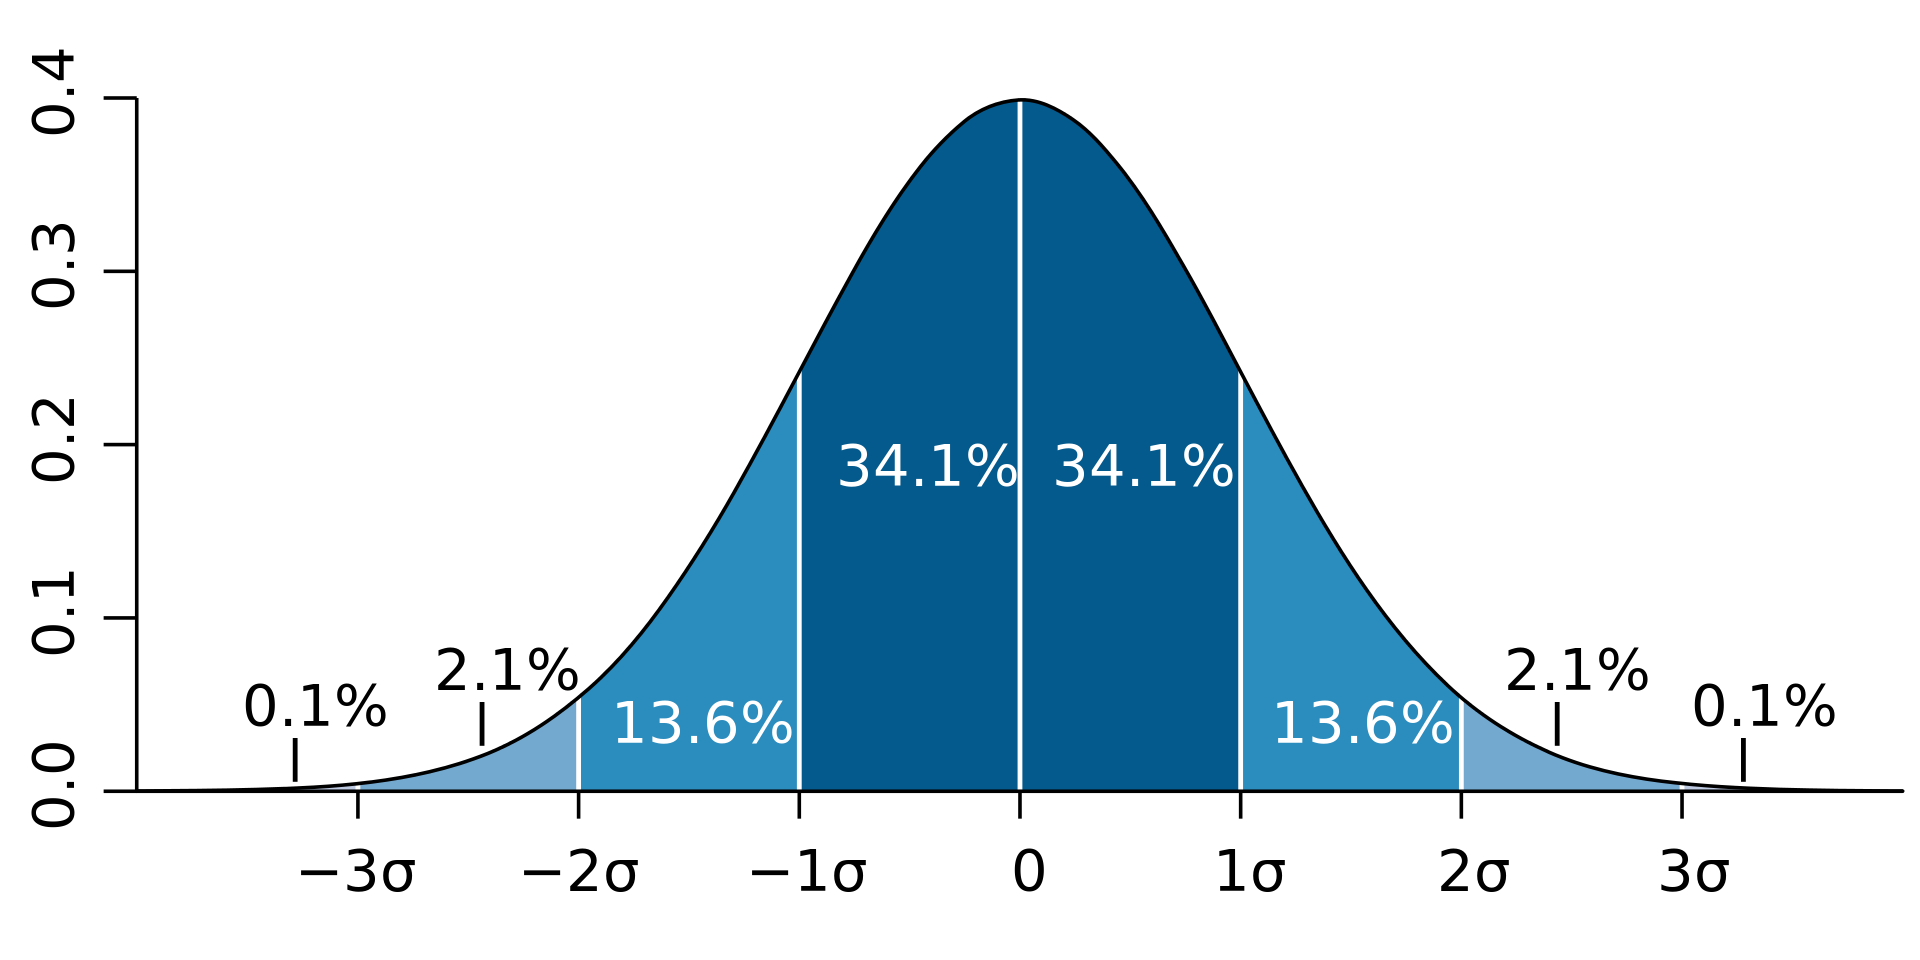
\includegraphics[width=0.5\textwidth]{images/Normalverteilung.png}
    \caption{Intervalle um den Mittelwert einer Normalverteilung \cite{normalverteilung}}
    \label{fig:normalverteilung}
\end{figure}


\subsection{R und RStudio}

R ist eine im Jahr 1992 entwickelte Programmiersprche bzw.- umgebung, um statistische Auswertungen und Grafiken zu erzeugen. Sie enthält bereits viele Funktionen zu diesem Zweck, kann aber auch sehr leicht durch Bibliotheken erweitert werden. Auswertungen und Grafiken haben eine entsprechende Qualität, um direkt in Veröffentlichungen genutzt zu werden. Insbesondere für sich wiederholende Auswertungen kann es sehr sinnvoll sein, eigene Skripte mit R zu schreiben und diese wiederholt auszuführen. Daten können beispielsweise sehr leicht aus gängigen Datenformaten wie CSV importiert und verarbeitet werden. Die Sprache hat eine relativ große Bekanntheit und Community, was eine Entwicklung und das finden von speziellen Lösungen sehr einfach macht. \cite{r}

RStudio ist eine für R entwickelte Entwicklungsumgebung, die eine einfachere Handhabung möglich macht. Eine grafische Benutzeroberfläche, Syntaxhighlighting, automatische Codeeinrückung o.ä., wie es aus Entwicklungsumgebungen vieler anderer Sprachen bekannt ist, machen die Bedienung sehr viel einfacher, als es noch zum Beginn der Entwicklung von R der Fall war. \cite{rstudio}


